\section{Burger's Equation}
In this problem you will solve Burgers equation, $u_t+f_x= 0,\ f=\frac{1}{2}u^2,\ x \in [0,4)$, periodic boundaries, with the initial condition shown below.

\begin{figure}[h]
    \centering
    

\tikzset{every picture/.style={line width=0.75pt}} %set default line width to 0.75pt        

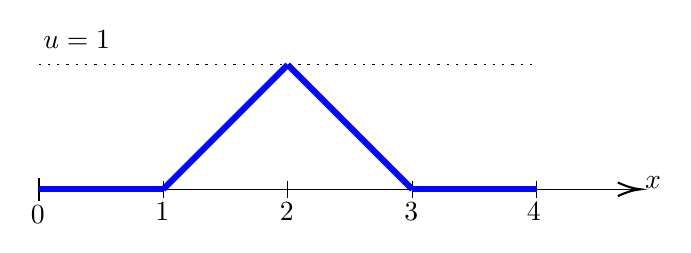
\begin{tikzpicture}[x=0.75pt,y=0.75pt,yscale=-1,xscale=1]
%uncomment if require: \path (0,300); %set diagram left start at 0, and has height of 300

%Straight Lines [id:da7588090942261074] 
\draw    (170,140) -- (458,140) (230,136) -- (230,144)(290,136) -- (290,144)(350,136) -- (350,144)(410,136) -- (410,144) ;
\draw [shift={(460,140)}, rotate = 180] [color={rgb, 255:red, 0; green, 0; blue, 0 }  ][line width=0.75]    (10.93,-3.29) .. controls (6.95,-1.4) and (3.31,-0.3) .. (0,0) .. controls (3.31,0.3) and (6.95,1.4) .. (10.93,3.29)   ;
\draw [shift={(170,140)}, rotate = 180] [color={rgb, 255:red, 0; green, 0; blue, 0 }  ][line width=0.75]    (0,5.59) -- (0,-5.59)   ;
%Straight Lines [id:da5719850269486109] 
\draw [color={rgb, 255:red, 2; green, 7; blue, 255 }  ,draw opacity=1 ][line width=2.25]    (170,140) -- (230,140) ;
%Straight Lines [id:da39606160939166957] 
\draw [color={rgb, 255:red, 2; green, 7; blue, 255 }  ,draw opacity=1 ][line width=2.25]    (230,140) -- (290,80) ;
%Straight Lines [id:da34987570129962964] 
\draw [color={rgb, 255:red, 2; green, 7; blue, 255 }  ,draw opacity=1 ][line width=2.25]    (290,80) -- (350,140) ;
%Straight Lines [id:da07428450981597945] 
\draw [color={rgb, 255:red, 2; green, 7; blue, 255 }  ,draw opacity=1 ][line width=2.25]    (350,140) -- (410,140) ;
%Straight Lines [id:da3360506402216956] 
\draw  [dash pattern={on 0.84pt off 2.51pt}]  (170,80) -- (410,80) ;

% Text Node
\draw (171,62.4) node [anchor=north west][inner sep=0.75pt]    {$u=1$};
% Text Node
\draw (461,132.4) node [anchor=north west][inner sep=0.75pt]    {$x$};
% Text Node
\draw (165,146.4) node [anchor=north west][inner sep=0.75pt]    {$0$};
% Text Node
\draw (225,145.4) node [anchor=north west][inner sep=0.75pt]    {$1$};
% Text Node
\draw (285,145.4) node [anchor=north west][inner sep=0.75pt]    {$2$};
% Text Node
\draw (345,145.4) node [anchor=north west][inner sep=0.75pt]    {$3$};
% Text Node
\draw (404,145.4) node [anchor=north west][inner sep=0.75pt]    {$4$};


\end{tikzpicture}

    \caption{Initial condition to Burgers equation.}
\end{figure}

For the numerical method, use the finite volume method (FVM) with $N_x$ uniform cells, forward Euler time stepping, a uniform time step, CFL=0.8 (based on the initial condition), and the upwind flux,

\begin{equation*}
    \hat{F}_{j + \frac{1}{2}} = \frac{1}{2}\left(f_j + f_{j+1}\right) - \frac{1}{2}|\hat{a}_{j + \frac{1}{2}}|\left(u_{j+1} - u_j\right)
\end{equation*}

\begin{enumerate}[label=\alph*., start = 1]
    \item Prior to implementing the FVM, determine the analytical solution using the method of characteristics. Plot the state, $u(x,t)$, at times $t= 0.5,\ 1.0,\ 1.5$ in one figure. In a separate figure, make a space-time diagram of the characteristics, up to $t= 1.5$, and indicate any shock speeds/paths.

\end{enumerate}
    
\begin{enumerate}[label=\alph*., start = 2]
    \item Implement the FVM and using $N_x$= 128 and $N_x$= 512, show the states at the same times as requested in the previous part. Make three plots, one for each time, and overlay the two $N_x$ results and the analytical solution on each plot. Comment on the differences.
\end{enumerate}
    
\begin{enumerate}[label=\alph*., start = 3]
    \item Perform a convergence study of the FVM, using the $L_2$ solution error norm at $t = 0.5$, for $N_x= 128,\ 256,\ 512,\ 1024.$  Include an error convergence plot and compute/discuss the rate.
\end{enumerate}
